\documentclass[30pt,twocolumn,letterpaper]{article}
\usepackage{cvpr}
\usepackage{times}
\usepackage{booktabs}
\usepackage{epsfig}
\usepackage{graphicx}
\usepackage{amsmath}
\usepackage{amssymb}
\cvprfinalcopy
\def\cvprPaperID{****}
\def\httilde{\mbox{\tt\raisebox{-.5ex}{\symbol{126}}}}
\usepackage{graphicx}
\usepackage{indentfirst}
\setlength{\parindent}{2em}
\usepackage{cite}
\usepackage[colorlinks,linkcolor=red,anchorcolor=blue,citecolor=green,backref=page]{hyperref}
\author{Qilei Zhang\\\\
Jun 26 2018}
\title{Instance-sensitive Fully Convolutional Networks}
\begin{document}
\maketitle
\begin{abstract}
  Fully convolutional networks have been proven very successful for semantic segmentation, but the FCN outputs are unaware of object instances.
\end{abstract}
\section{Introduction}
Fully convolutional networks have been proven an effective end-to-end solution to semantic image segmentation. An FCN produces a score map of a size proportional to the input image, where every pixel represents a classifier of objects.Despite good accuracy and ease of usage, FCNs are not directly applicable for producing instance segments\cite{Carson1981Some}. \\
\begin{figure}[htbp]
\small
\centering
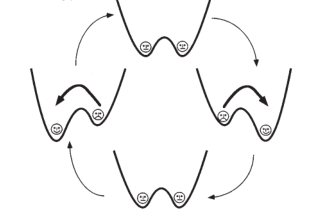
\includegraphics[width=20em]{000.png}
\caption{Methodological comparisons between: (top)FCN for semantic segmentation;
(bottom) our Instance FCN for instance segment proposal.}
\label{fig:lable}
\end{figure}\\
\section{Related Work}
For the convolution neural network,the sliding window does not necessarily run on the image domain, but runs on the feature mapping\cite{Heimer2011Disarticulated}, and the feature mapping can be re convoluted into a convolution filter on the feature mapping\cite{Ljungqvist2000Firm}.FCNs have shown compelling quality and efficiency for semantic segmentation. Each output pixel is a classifier corresponding to the receptive field of the network.The networks can thus be trained end-to-end, pixel-to-pixel, given the category-wise semantic segmentation annotation. But this can not distinguish object instances. \\
\begin{figure}[htbp]
\small
\centering
\includegraphics[width=20em]{001.png}
\caption{Methodological comparisons between DeepMask and InstanceFCN for
instance segment proposal.}
\label{fig:lable}
\end{figure}\\
\section{Conclusion}
FCN is driven by classifying pixels based on their relative positions, which leads to a set of instance-sensitive score maps. A simple assembling module is then able to generate segment instances from these score maps\cite{Pereira2015Empirical}.
{\small
\bibliographystyle{ieee}
\bibliography{1}
}
\end{document}
